\documentclass[11pt,letterpaper]{article}
\usepackage[utf8]{inputenc}
\usepackage{amsmath,amssymb,fullpage,graphicx}
\usepackage{subfigure}
\let\hat\widehat
\let\tilde\widetilde

\begin{document}
\section*{Q1}
\subsection*{Q1-a}
\begin{verbatim}
n <- 100
mu <- 5
sample_dt <- rnorm(n, mu, 1)

> summary(sample_dt)
   Min. 1st Qu.  Median    Mean 3rd Qu.    Max. 
  2.757   4.368   4.955   5.085   5.875   7.455 
\end{verbatim}

\subsection*{Q1-b}
\noindent Rewrite the prior as normal prior with density $\pi(\theta) \sim N(\theta_0, \tau_0^2)$ where $\tau_0^2 = \infty$. \\

\noindent The likelihood function is
\begin{align*}
L(\theta | x_1...x_n) = (\frac{1}{\sqrt{2 \pi \sigma^2}})^n e^{\frac{-1}{2 \sigma^2} \sum_0^n (x_i - \theta)^2 }
\end{align*}

\begin{align*}
\sum_0^n (x_i - \theta)^2 &= \sum (x_i - \bar{x} + \bar{x} - \theta)^2 \\
&= \sum (x_i - \bar{x})^2 + (\bar{x} - \theta)^2 
\end{align*}
\noindent Since $\sum (x_i - \bar{x})(\bar{x} - \theta) = 0$
\begin{align*}
\text{define: } s^2 &= \frac{1}{n} \sum (x_i - \bar{x})^2 \\
\sum_0^n (x_i - \theta)^2 &= ns^2 + n(\bar{x} - \theta)^2
\end{align*}
\noindent The posterior function is
\begin{align*}
\pi(\theta | x_1...x_n) &= L(\theta | x_1...x_n) \pi(\theta) \\
&\propto e^{-\frac{1}{2 \sigma^2}(ns^2 + n(\bar{x} - \theta))^2} e^{-\frac{1}{2 \tau_0^2}(\theta - \theta_0)^2} \\
&\propto e^{-\frac{n}{2 \sigma^2}(s^2 + (\bar{x} - \theta))^2} e^{-\frac{1}{2 \tau_0^2}(\theta - \theta_0)^2} 
\end{align*}
\begin{align*}
\text{define: } \tau_1^2 &= (\frac{1}{\tau_0^2} + \frac{n}{\sigma^2})^{-1} \\
w &= \frac{\frac{n}{\sigma^2}}{\frac{n}{\sigma^2} + \frac{1}{\tau_0^2}} \\
\theta_1 &= w\bar{X} + (1-w)\theta_0
\end{align*}
Then the posterior function can be represented as 
\begin{align*}
\pi(\theta | x_1...x_n) \propto e^{-\frac{1}{2 \tau_1^2}(\theta - \theta_1)^2 }
\end{align*}
\noindent Right hand side of this formula is part of normal density function. Thus, the posterior function follows normal distribution $N(\theta_1, \tau_1^2)$
\begin{align*}
w &= \frac{\frac{n}{\sigma^2}}{\frac{n}{\sigma^2} + \frac{1}{\tau_0^2}} \text{, } \sigma = 1 \text{, } \tau_0^2 = \infty \\
w &= \frac{n}{n + 0} = 1 \\
\theta_1 &= \bar{X} \\
\tau_1^2 &= (\frac{1}{\tau_0^2} + \frac{n}{\sigma^2} )^{-1} \text{, } \tau_0^2 = \infty \text{, } \sigma = 1\\
\tau_1^2 &= \frac{1}{n}
\end{align*}
\noindent In this case, we get mean and variance of the posterior are $\bar{X}$ and $\frac{1}{n}$. The exact density function of posterior can be written as
\begin{align*}
\pi(\theta | x_1...x_n) &= \frac{1}{\sqrt{2 \pi \tau_1^2}} e^{-\frac{1}{2 \tau_1^2}(\theta - \theta_1)^2} \\
&= \frac{\sqrt{n}}{\sqrt{2 \pi}} e^{-\frac{n}{2}(\theta - \bar{X})^2}
\end{align*}

\noindent Based on the sample data generated in previous question, where $n = 100$ and $\bar{X} = 5.085$. \\
\noindent $\pi(\theta | x_1...x_n) \sim N(5.085, 0.01)$

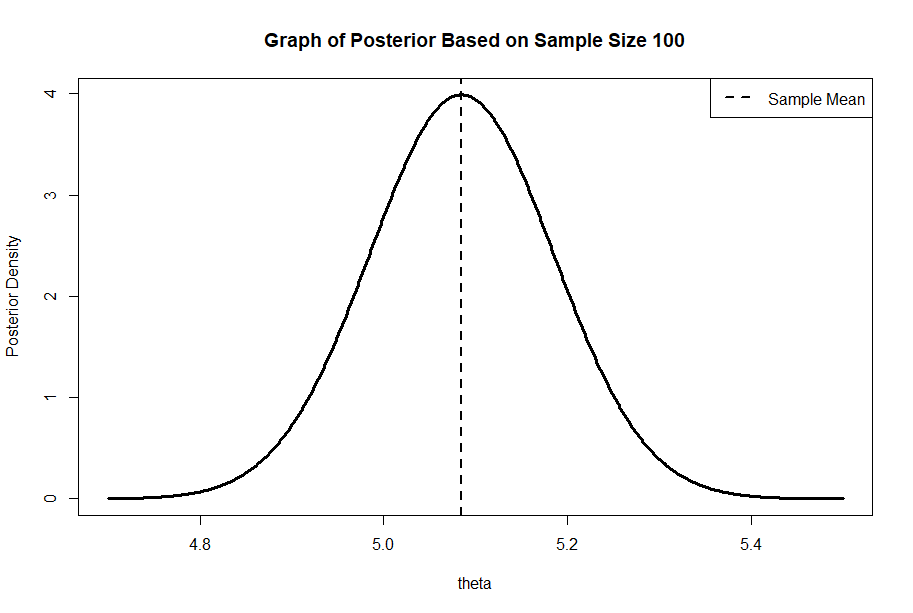
\includegraphics[width=150mm]{posterior_density.png}

\subsection*{Q1-c}
\noindent The posterior distribution of $\theta$ follows normal distribution with mean $\bar{X} = 5.085$ and variance $\frac{1}{n} = 0.01$, therefore
\begin{align*}
\frac{\theta - \mathbb{E}(\theta | \bar{X})}{Var(\theta | \bar{X})} \sim N(0, 1))
\end{align*}
\noindent $95 \%$ credible interval for $\theta$ can be represented by 
\begin{align*}
95 \% CI &= P(L(\bar{X} < \theta < U(\bar{X}))) \\
&= [\mathbb{E}(\theta | \bar{X}) - Z_{\frac{0.05}{2}} \sqrt{Var(\theta | \bar{X})} \text{,  }  \mathbb{E}(\theta | \bar{X}) + Z_{\frac{0.05}{2}} \sqrt{Var(\theta | \bar{X})} ] \\
&= [5.085 - 1.96 \cdot 0.1 \text{,  } 5.085 + 1.96 \cdot 0.1] \\
&= [4.889 \text{,  } 5.281]
\end{align*}

\noindent Given the sample data, the probability that true $\theta$ falls in between 4.889 and 5.281 is 0.95.

\subsection*{Q1-d}
\begin{verbatim}
post_mu <- 5.085
post_sigma <- sqrt(1/100)
theta_dt <- rnorm(1000, post_mu, post_sigma)

theta_value <- seq(4.7, 5.5, 0.001)
post_density <- dnorm(theta_value, post_mu, post_sigma)

hist(theta_dt, breaks=20, probability=T, main='Histogram of Theta', 
     xlab='theta', ylab='Density')
lines(theta_value, post_density, lwd=3)
legend('topright', 'Posterior Density', lty=1, lwd=3, cex=1)
\end{verbatim}
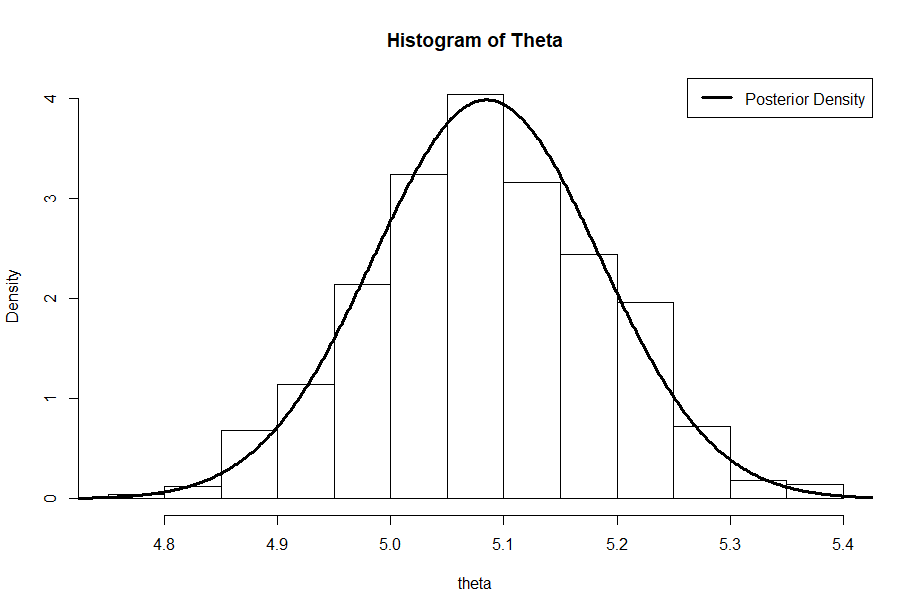
\includegraphics[width=150mm]{hist_theta.png}

\subsection*{Q1-e}
\begin{verbatim}
> quantile(theta_dt, 0.025)
   2.5% 
4.88424 
> quantile(theta_dt, 0.975)
   97.5% 
5.280327 
\end{verbatim}

\noindent The lower bound is 4.88424, and the upper bound is 5.280327. The interval captured from simulated data is approximately identical to calculated credible interval in previous question.



\end{document}